% Created by tikzDevice version 0.12.6 on 2026-04-25 20:39:56
% !TEX encoding = UTF-8 Unicode
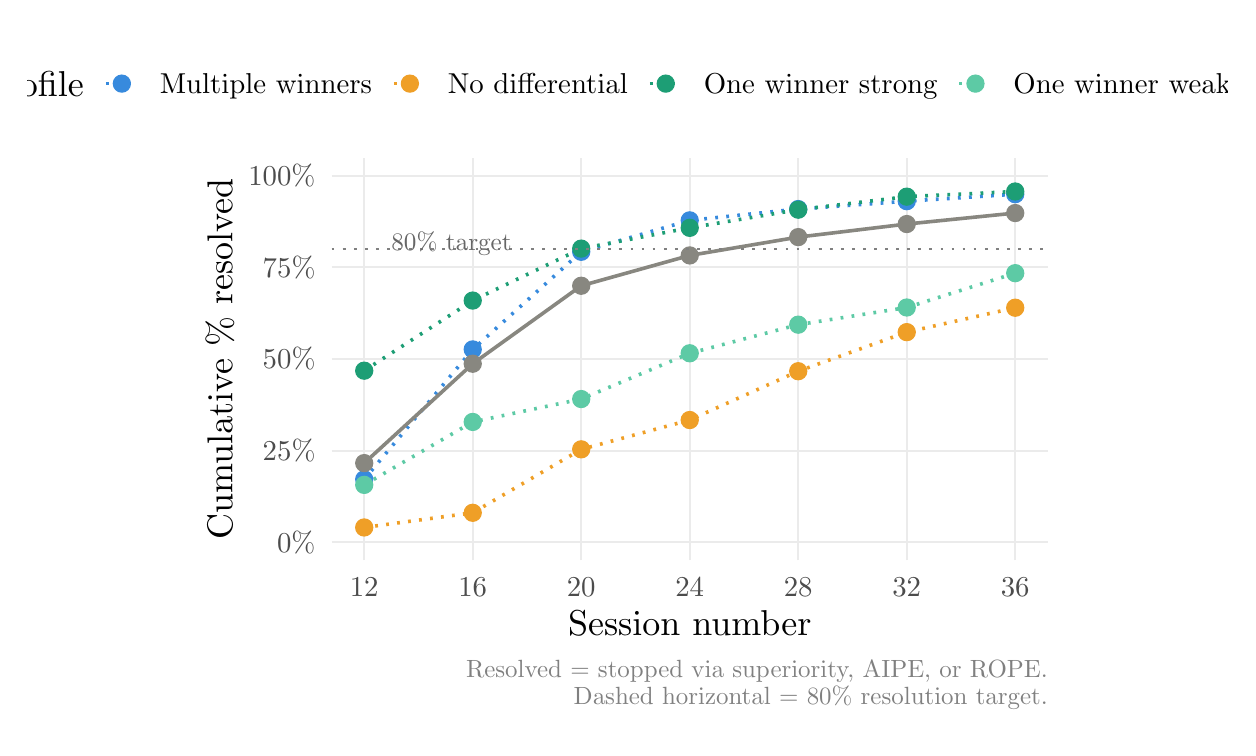
\begin{tikzpicture}[x=1pt,y=1pt]
\definecolor{fillColor}{RGB}{255,255,255}
\path[use as bounding box,fill=fillColor,fill opacity=0.00] (0,0) rectangle (433.62,252.94);
\begin{scope}
\path[clip] ( 58.50,  0.00) rectangle (375.12,252.94);
\definecolor{fillColor}{RGB}{255,255,255}

\path[fill=fillColor] ( 58.50,  0.00) rectangle (375.12,252.94);
\end{scope}
\begin{scope}
\path[clip] (109.85, 60.43) rectangle (368.62,205.99);
\definecolor{drawColor}{gray}{0.92}

\path[draw=drawColor,line width= 0.7pt,line join=round] (109.85, 67.05) --
	(368.62, 67.05);

\path[draw=drawColor,line width= 0.7pt,line join=round] (109.85,100.13) --
	(368.62,100.13);

\path[draw=drawColor,line width= 0.7pt,line join=round] (109.85,133.21) --
	(368.62,133.21);

\path[draw=drawColor,line width= 0.7pt,line join=round] (109.85,166.29) --
	(368.62,166.29);

\path[draw=drawColor,line width= 0.7pt,line join=round] (109.85,199.37) --
	(368.62,199.37);

\path[draw=drawColor,line width= 0.7pt,line join=round] (121.61, 60.43) --
	(121.61,205.99);

\path[draw=drawColor,line width= 0.7pt,line join=round] (160.82, 60.43) --
	(160.82,205.99);

\path[draw=drawColor,line width= 0.7pt,line join=round] (200.02, 60.43) --
	(200.02,205.99);

\path[draw=drawColor,line width= 0.7pt,line join=round] (239.23, 60.43) --
	(239.23,205.99);

\path[draw=drawColor,line width= 0.7pt,line join=round] (278.44, 60.43) --
	(278.44,205.99);

\path[draw=drawColor,line width= 0.7pt,line join=round] (317.65, 60.43) --
	(317.65,205.99);

\path[draw=drawColor,line width= 0.7pt,line join=round] (356.85, 60.43) --
	(356.85,205.99);
\definecolor{drawColor}{RGB}{55,138,221}

\path[draw=drawColor,line width= 1.3pt,dash pattern=on 1pt off 3pt ,line join=round] (121.61, 89.73) --
	(160.82,136.68) --
	(200.02,171.96) --
	(239.23,183.31) --
	(278.44,187.40) --
	(317.65,190.24) --
	(356.85,192.76);
\definecolor{drawColor}{RGB}{239,159,39}

\path[draw=drawColor,line width= 1.3pt,dash pattern=on 1pt off 3pt ,line join=round] (121.61, 72.34) --
	(160.82, 77.64) --
	(200.02,100.57) --
	(239.23,111.16) --
	(278.44,128.80) --
	(317.65,142.92) --
	(356.85,151.74);
\definecolor{drawColor}{RGB}{29,158,117}

\path[draw=drawColor,line width= 1.3pt,dash pattern=on 1pt off 3pt ,line join=round] (121.61,128.99) --
	(160.82,154.33) --
	(200.02,173.10) --
	(239.23,180.61) --
	(278.44,187.17) --
	(317.65,191.87) --
	(356.85,193.74);
\definecolor{drawColor}{RGB}{93,202,165}

\path[draw=drawColor,line width= 1.3pt,dash pattern=on 1pt off 3pt ,line join=round] (121.61, 87.73) --
	(160.82,110.47) --
	(200.02,118.74) --
	(239.23,135.28) --
	(278.44,145.62) --
	(317.65,151.82) --
	(356.85,164.23);
\definecolor{drawColor}{RGB}{136,135,128}

\path[draw=drawColor,line width= 1.3pt,line join=round] (121.61, 95.59) --
	(160.82,131.51) --
	(200.02,159.68) --
	(239.23,170.64) --
	(278.44,177.26) --
	(317.65,181.98) --
	(356.85,185.95);
\definecolor{drawColor}{RGB}{55,138,221}
\definecolor{fillColor}{RGB}{55,138,221}

\path[draw=drawColor,line width= 0.4pt,line join=round,line cap=round,fill=fillColor] (121.61, 89.73) circle (  3.10);
\definecolor{drawColor}{RGB}{239,159,39}
\definecolor{fillColor}{RGB}{239,159,39}

\path[draw=drawColor,line width= 0.4pt,line join=round,line cap=round,fill=fillColor] (121.61, 72.34) circle (  3.10);
\definecolor{drawColor}{RGB}{29,158,117}
\definecolor{fillColor}{RGB}{29,158,117}

\path[draw=drawColor,line width= 0.4pt,line join=round,line cap=round,fill=fillColor] (121.61,128.99) circle (  3.10);
\definecolor{drawColor}{RGB}{93,202,165}
\definecolor{fillColor}{RGB}{93,202,165}

\path[draw=drawColor,line width= 0.4pt,line join=round,line cap=round,fill=fillColor] (121.61, 87.73) circle (  3.10);
\definecolor{drawColor}{RGB}{55,138,221}
\definecolor{fillColor}{RGB}{55,138,221}

\path[draw=drawColor,line width= 0.4pt,line join=round,line cap=round,fill=fillColor] (160.82,136.68) circle (  3.10);
\definecolor{drawColor}{RGB}{239,159,39}
\definecolor{fillColor}{RGB}{239,159,39}

\path[draw=drawColor,line width= 0.4pt,line join=round,line cap=round,fill=fillColor] (160.82, 77.64) circle (  3.10);
\definecolor{drawColor}{RGB}{29,158,117}
\definecolor{fillColor}{RGB}{29,158,117}

\path[draw=drawColor,line width= 0.4pt,line join=round,line cap=round,fill=fillColor] (160.82,154.33) circle (  3.10);
\definecolor{drawColor}{RGB}{93,202,165}
\definecolor{fillColor}{RGB}{93,202,165}

\path[draw=drawColor,line width= 0.4pt,line join=round,line cap=round,fill=fillColor] (160.82,110.47) circle (  3.10);
\definecolor{drawColor}{RGB}{55,138,221}
\definecolor{fillColor}{RGB}{55,138,221}

\path[draw=drawColor,line width= 0.4pt,line join=round,line cap=round,fill=fillColor] (200.02,171.96) circle (  3.10);
\definecolor{drawColor}{RGB}{239,159,39}
\definecolor{fillColor}{RGB}{239,159,39}

\path[draw=drawColor,line width= 0.4pt,line join=round,line cap=round,fill=fillColor] (200.02,100.57) circle (  3.10);
\definecolor{drawColor}{RGB}{29,158,117}
\definecolor{fillColor}{RGB}{29,158,117}

\path[draw=drawColor,line width= 0.4pt,line join=round,line cap=round,fill=fillColor] (200.02,173.10) circle (  3.10);
\definecolor{drawColor}{RGB}{93,202,165}
\definecolor{fillColor}{RGB}{93,202,165}

\path[draw=drawColor,line width= 0.4pt,line join=round,line cap=round,fill=fillColor] (200.02,118.74) circle (  3.10);
\definecolor{drawColor}{RGB}{55,138,221}
\definecolor{fillColor}{RGB}{55,138,221}

\path[draw=drawColor,line width= 0.4pt,line join=round,line cap=round,fill=fillColor] (239.23,183.31) circle (  3.10);
\definecolor{drawColor}{RGB}{239,159,39}
\definecolor{fillColor}{RGB}{239,159,39}

\path[draw=drawColor,line width= 0.4pt,line join=round,line cap=round,fill=fillColor] (239.23,111.16) circle (  3.10);
\definecolor{drawColor}{RGB}{29,158,117}
\definecolor{fillColor}{RGB}{29,158,117}

\path[draw=drawColor,line width= 0.4pt,line join=round,line cap=round,fill=fillColor] (239.23,180.61) circle (  3.10);
\definecolor{drawColor}{RGB}{93,202,165}
\definecolor{fillColor}{RGB}{93,202,165}

\path[draw=drawColor,line width= 0.4pt,line join=round,line cap=round,fill=fillColor] (239.23,135.28) circle (  3.10);
\definecolor{drawColor}{RGB}{55,138,221}
\definecolor{fillColor}{RGB}{55,138,221}

\path[draw=drawColor,line width= 0.4pt,line join=round,line cap=round,fill=fillColor] (278.44,187.40) circle (  3.10);
\definecolor{drawColor}{RGB}{239,159,39}
\definecolor{fillColor}{RGB}{239,159,39}

\path[draw=drawColor,line width= 0.4pt,line join=round,line cap=round,fill=fillColor] (278.44,128.80) circle (  3.10);
\definecolor{drawColor}{RGB}{29,158,117}
\definecolor{fillColor}{RGB}{29,158,117}

\path[draw=drawColor,line width= 0.4pt,line join=round,line cap=round,fill=fillColor] (278.44,187.17) circle (  3.10);
\definecolor{drawColor}{RGB}{93,202,165}
\definecolor{fillColor}{RGB}{93,202,165}

\path[draw=drawColor,line width= 0.4pt,line join=round,line cap=round,fill=fillColor] (278.44,145.62) circle (  3.10);
\definecolor{drawColor}{RGB}{55,138,221}
\definecolor{fillColor}{RGB}{55,138,221}

\path[draw=drawColor,line width= 0.4pt,line join=round,line cap=round,fill=fillColor] (317.65,190.24) circle (  3.10);
\definecolor{drawColor}{RGB}{239,159,39}
\definecolor{fillColor}{RGB}{239,159,39}

\path[draw=drawColor,line width= 0.4pt,line join=round,line cap=round,fill=fillColor] (317.65,142.92) circle (  3.10);
\definecolor{drawColor}{RGB}{29,158,117}
\definecolor{fillColor}{RGB}{29,158,117}

\path[draw=drawColor,line width= 0.4pt,line join=round,line cap=round,fill=fillColor] (317.65,191.87) circle (  3.10);
\definecolor{drawColor}{RGB}{93,202,165}
\definecolor{fillColor}{RGB}{93,202,165}

\path[draw=drawColor,line width= 0.4pt,line join=round,line cap=round,fill=fillColor] (317.65,151.82) circle (  3.10);
\definecolor{drawColor}{RGB}{55,138,221}
\definecolor{fillColor}{RGB}{55,138,221}

\path[draw=drawColor,line width= 0.4pt,line join=round,line cap=round,fill=fillColor] (356.85,192.76) circle (  3.10);
\definecolor{drawColor}{RGB}{239,159,39}
\definecolor{fillColor}{RGB}{239,159,39}

\path[draw=drawColor,line width= 0.4pt,line join=round,line cap=round,fill=fillColor] (356.85,151.74) circle (  3.10);
\definecolor{drawColor}{RGB}{29,158,117}
\definecolor{fillColor}{RGB}{29,158,117}

\path[draw=drawColor,line width= 0.4pt,line join=round,line cap=round,fill=fillColor] (356.85,193.74) circle (  3.10);
\definecolor{drawColor}{RGB}{93,202,165}
\definecolor{fillColor}{RGB}{93,202,165}

\path[draw=drawColor,line width= 0.4pt,line join=round,line cap=round,fill=fillColor] (356.85,164.23) circle (  3.10);
\definecolor{drawColor}{RGB}{136,135,128}
\definecolor{fillColor}{RGB}{136,135,128}

\path[draw=drawColor,line width= 0.4pt,line join=round,line cap=round,fill=fillColor] (121.61, 95.59) circle (  3.10);

\path[draw=drawColor,line width= 0.4pt,line join=round,line cap=round,fill=fillColor] (160.82,131.51) circle (  3.10);

\path[draw=drawColor,line width= 0.4pt,line join=round,line cap=round,fill=fillColor] (200.02,159.68) circle (  3.10);

\path[draw=drawColor,line width= 0.4pt,line join=round,line cap=round,fill=fillColor] (239.23,170.64) circle (  3.10);

\path[draw=drawColor,line width= 0.4pt,line join=round,line cap=round,fill=fillColor] (278.44,177.26) circle (  3.10);

\path[draw=drawColor,line width= 0.4pt,line join=round,line cap=round,fill=fillColor] (317.65,181.98) circle (  3.10);

\path[draw=drawColor,line width= 0.4pt,line join=round,line cap=round,fill=fillColor] (356.85,185.95) circle (  3.10);
\definecolor{drawColor}{gray}{0.50}

\path[draw=drawColor,line width= 0.7pt,dash pattern=on 1pt off 3pt ,line join=round] (109.85,172.91) -- (368.62,172.91);
\definecolor{drawColor}{gray}{0.40}

\node[text=drawColor,anchor=base west,inner sep=0pt, outer sep=0pt, scale=  0.91] at (131.41,172.42) {80\% target};
\end{scope}
\begin{scope}
\path[clip] (  0.00,  0.00) rectangle (433.62,252.94);
\definecolor{drawColor}{gray}{0.30}

\node[text=drawColor,anchor=base east,inner sep=0pt, outer sep=0pt, scale=  1.04] at (104.00, 63.47) {0\%};

\node[text=drawColor,anchor=base east,inner sep=0pt, outer sep=0pt, scale=  1.04] at (104.00, 96.55) {25\%};

\node[text=drawColor,anchor=base east,inner sep=0pt, outer sep=0pt, scale=  1.04] at (104.00,129.63) {50\%};

\node[text=drawColor,anchor=base east,inner sep=0pt, outer sep=0pt, scale=  1.04] at (104.00,162.71) {75\%};

\node[text=drawColor,anchor=base east,inner sep=0pt, outer sep=0pt, scale=  1.04] at (104.00,195.79) {100\%};
\end{scope}
\begin{scope}
\path[clip] (  0.00,  0.00) rectangle (433.62,252.94);
\definecolor{drawColor}{gray}{0.30}

\node[text=drawColor,anchor=base,inner sep=0pt, outer sep=0pt, scale=  1.04] at (121.61, 47.42) {12};

\node[text=drawColor,anchor=base,inner sep=0pt, outer sep=0pt, scale=  1.04] at (160.82, 47.42) {16};

\node[text=drawColor,anchor=base,inner sep=0pt, outer sep=0pt, scale=  1.04] at (200.02, 47.42) {20};

\node[text=drawColor,anchor=base,inner sep=0pt, outer sep=0pt, scale=  1.04] at (239.23, 47.42) {24};

\node[text=drawColor,anchor=base,inner sep=0pt, outer sep=0pt, scale=  1.04] at (278.44, 47.42) {28};

\node[text=drawColor,anchor=base,inner sep=0pt, outer sep=0pt, scale=  1.04] at (317.65, 47.42) {32};

\node[text=drawColor,anchor=base,inner sep=0pt, outer sep=0pt, scale=  1.04] at (356.85, 47.42) {36};
\end{scope}
\begin{scope}
\path[clip] (  0.00,  0.00) rectangle (433.62,252.94);
\definecolor{drawColor}{RGB}{0,0,0}

\node[text=drawColor,anchor=base,inner sep=0pt, outer sep=0pt, scale=  1.30] at (239.23, 33.20) {Session number};
\end{scope}
\begin{scope}
\path[clip] (  0.00,  0.00) rectangle (433.62,252.94);
\definecolor{drawColor}{RGB}{0,0,0}

\node[text=drawColor,rotate= 90.00,anchor=base,inner sep=0pt, outer sep=0pt, scale=  1.30] at ( 73.96,133.21) {Cumulative \% resolved};
\end{scope}
\begin{scope}
\path[clip] (  0.00,  0.00) rectangle (433.62,252.94);
\definecolor{drawColor}{RGB}{0,0,0}

\node[text=drawColor,anchor=base west,inner sep=0pt, outer sep=0pt, scale=  1.30] at (-16.74,228.24) {Profile};
\end{scope}
\begin{scope}
\path[clip] (  0.00,  0.00) rectangle (433.62,252.94);
\definecolor{drawColor}{RGB}{55,138,221}

\path[draw=drawColor,line width= 1.3pt,dash pattern=on 1pt off 3pt ,line join=round] ( 28.25,232.72) -- ( 39.81,232.72);
\definecolor{fillColor}{RGB}{55,138,221}

\path[draw=drawColor,line width= 0.4pt,line join=round,line cap=round,fill=fillColor] ( 34.03,232.72) circle (  3.10);
\end{scope}
\begin{scope}
\path[clip] (  0.00,  0.00) rectangle (433.62,252.94);
\definecolor{drawColor}{RGB}{239,159,39}

\path[draw=drawColor,line width= 1.3pt,dash pattern=on 1pt off 3pt ,line join=round] (132.33,232.72) -- (143.89,232.72);
\definecolor{fillColor}{RGB}{239,159,39}

\path[draw=drawColor,line width= 0.4pt,line join=round,line cap=round,fill=fillColor] (138.11,232.72) circle (  3.10);
\end{scope}
\begin{scope}
\path[clip] (  0.00,  0.00) rectangle (433.62,252.94);
\definecolor{drawColor}{RGB}{29,158,117}

\path[draw=drawColor,line width= 1.3pt,dash pattern=on 1pt off 3pt ,line join=round] (224.79,232.72) -- (236.36,232.72);
\definecolor{fillColor}{RGB}{29,158,117}

\path[draw=drawColor,line width= 0.4pt,line join=round,line cap=round,fill=fillColor] (230.57,232.72) circle (  3.10);
\end{scope}
\begin{scope}
\path[clip] (  0.00,  0.00) rectangle (433.62,252.94);
\definecolor{drawColor}{RGB}{93,202,165}

\path[draw=drawColor,line width= 1.3pt,dash pattern=on 1pt off 3pt ,line join=round] (336.70,232.72) -- (348.26,232.72);
\definecolor{fillColor}{RGB}{93,202,165}

\path[draw=drawColor,line width= 0.4pt,line join=round,line cap=round,fill=fillColor] (342.48,232.72) circle (  3.10);
\end{scope}
\begin{scope}
\path[clip] (  0.00,  0.00) rectangle (433.62,252.94);
\definecolor{drawColor}{RGB}{136,135,128}

\path[draw=drawColor,line width= 1.3pt,line join=round] (442.74,232.72) -- (454.30,232.72);
\definecolor{fillColor}{RGB}{136,135,128}

\path[draw=drawColor,line width= 0.4pt,line join=round,line cap=round,fill=fillColor] (448.52,232.72) circle (  3.10);
\end{scope}
\begin{scope}
\path[clip] (  0.00,  0.00) rectangle (433.62,252.94);
\definecolor{drawColor}{RGB}{0,0,0}

\node[text=drawColor,anchor=base west,inner sep=0pt, outer sep=0pt, scale=  1.04] at ( 47.76,229.14) {Multiple winners};
\end{scope}
\begin{scope}
\path[clip] (  0.00,  0.00) rectangle (433.62,252.94);
\definecolor{drawColor}{RGB}{0,0,0}

\node[text=drawColor,anchor=base west,inner sep=0pt, outer sep=0pt, scale=  1.04] at (151.83,229.14) {No differential};
\end{scope}
\begin{scope}
\path[clip] (  0.00,  0.00) rectangle (433.62,252.94);
\definecolor{drawColor}{RGB}{0,0,0}

\node[text=drawColor,anchor=base west,inner sep=0pt, outer sep=0pt, scale=  1.04] at (244.30,229.14) {One winner strong};
\end{scope}
\begin{scope}
\path[clip] (  0.00,  0.00) rectangle (433.62,252.94);
\definecolor{drawColor}{RGB}{0,0,0}

\node[text=drawColor,anchor=base west,inner sep=0pt, outer sep=0pt, scale=  1.04] at (356.20,229.14) {One winner weak};
\end{scope}
\begin{scope}
\path[clip] (  0.00,  0.00) rectangle (433.62,252.94);
\definecolor{drawColor}{RGB}{0,0,0}

\node[text=drawColor,anchor=base west,inner sep=0pt, outer sep=0pt, scale=  1.04] at (462.25,229.14) {Overall};
\end{scope}
\begin{scope}
\path[clip] (  0.00,  0.00) rectangle (433.62,252.94);
\definecolor{drawColor}{gray}{0.50}

\node[text=drawColor,anchor=base east,inner sep=0pt, outer sep=0pt, scale=  0.90] at (368.62, 17.97) {Resolved = stopped via superiority, AIPE, or ROPE.};

\node[text=drawColor,anchor=base east,inner sep=0pt, outer sep=0pt, scale=  0.90] at (368.62,  8.25) {Dashed horizontal = 80\% resolution target.};
\end{scope}
\end{tikzpicture}
